\documentclass{beamer}
\mode<presentation>
\usepackage{amsmath}
\usepackage{amssymb}
%\usepackage{advdate}
\usepackage{adjustbox}
\usepackage{subcaption}
\usepackage{enumitem}
\usepackage{multicol}
\usepackage{mathtools}
\usepackage{listings} % For code formatting

\usepackage{url}
\def\UrlBreaks{\do\/\do-}
\usetheme{Boadilla}
\usecolortheme{lily}
\setbeamertemplate{footline}
{
  \leavevmode%
  \hbox{%
  \begin{beamercolorbox}[wd=\paperwidth,ht=2.25ex,dp=1ex,right]{author in head/foot}%
    \insertframenumber{} / \inserttotalframenumber\hspace*{2ex} 
  \end{beamercolorbox}}%
  \vskip0pt%
}
\setbeamertemplate{navigation symbols}{}

\providecommand{\nCr}[2]{\,^{#1}C_{#2}} % nCr
\providecommand{\nPr}[2]{\,^{#1}P_{#2}} % nPr
\providecommand{\mbf}{\mathbf}
\providecommand{\pr}[1]{\ensuremath{\Pr\left(#1\right)}}
\providecommand{\qfunc}[1]{\ensuremath{Q\left(#1\right)}}
\providecommand{\sbrak}[1]{\ensuremath{{}\left[#1\right]}}
\providecommand{\lsbrak}[1]{\ensuremath{{}\left[#1\right.}}
\providecommand{\rsbrak}[1]{\ensuremath{{}\left.#1\right]}}
\providecommand{\brak}[1]{\ensuremath{\left(#1\right)}}
\providecommand{\lbrak}[1]{\ensuremath{\left(#1\right.}}
\providecommand{\rbrak}[1]{\ensuremath{\left.#1\right)}}
\providecommand{\cbrak}[1]{\ensuremath{\left\{#1\right\}}}
\providecommand{\lcbrak}[1]{\ensuremath{\left\{#1\right.}}
\providecommand{\rcbrak}[1]{\ensuremath{\left.#1\right\}}}
\theoremstyle{remark}
\newtheorem{rem}{Remark}
\newcommand{\sgn}{\mathop{\mathrm{sgn}}}
\providecommand{\abs}[1]{\ensuremath{\left\lvert#1\right\rvert}}
\providecommand{\res}[1]{\Res\displaylimits_{#1}} 
\providecommand{\norm}[1]{\lVert#1\rVert}
\providecommand{\mtx}[1]{\mathbf{#1}}
\providecommand{\mean}[1]{\ensuremath{E\left[ #1 \right]}}
\providecommand{\fourier}{\overset{\mathcal{F}}{ \rightleftharpoons}}
%\providecommand{\hilbert}{\overset{\mathcal{H}}{ \rightleftharpoons}}
\providecommand{\system}{\overset{\mathcal{H}}{ \longleftrightarrow}}
	%\newcommand{\solution}[2]{\textbf{Solution:}{#1}}
%\newcommand{\solution}{\noindent \textbf{Solution: }}
\providecommand{\dec}[2]{\ensuremath{\overset{#1}{\underset{#2}{\gtrless}}}}
\newcommand{\myvec}[1]{\ensuremath{\begin{pmatrix}#1\end{pmatrix}}}
\let\vec\mathbf

\title{Assignment 3}
\author{Teja Vardhan Shannu}
\date{August 2024}

\begin{document}

\begin{frame}
\titlepage
\end{frame}

\begin{frame}
\frametitle{Problem Statement}
A line intersects the Y-axis and the X-axis at the points $ P\brak{0, b} $ and $ Q\brak{c, 0} $ respectively. If $ \brak{2, -5} $ is the midpoint of $ PQ $, find the coordinates of $ P $ and $ Q $.
\end{frame}

\begin{frame}
\frametitle{Problem Data}
\begin{table}[h]
\centering
\begin{tabular}{|c|c|}
\hline
\textbf{Point} & \textbf{Coordinates} \\ \hline
$ P $ & $ \begin{pmatrix} 0 \\ b \end{pmatrix} $ \\ \hline
$ Q $ & $ \begin{pmatrix} c \\ 0 \end{pmatrix} $ \\ \hline
$ M $ & $ \begin{pmatrix} 2 \\ -5 \end{pmatrix} $ \\ \hline
\end{tabular}
\end{table}
\end{frame}

\section{Solution}
\begin{frame}
\frametitle{Midpoint Formula}
Let the coordinates of points $ P $ and $ Q $ be:
\begin{equation*}
\mathbf{P} = \begin{pmatrix} 0 \\ b \end{pmatrix}, \quad \mathbf{Q} = \begin{pmatrix} c \\ 0 \end{pmatrix}
\end{equation*}
The midpoint $ M $ is given by:
\begin{equation*}
\mathbf{M} = \begin{pmatrix} 2 \\ -5 \end{pmatrix}
\end{equation*}
The midpoint formula states:
\begin{equation*}
\mathbf{M} = \frac{1}{2} \brak{\mathbf{P} + \mathbf{Q}}
\end{equation*}
\end{frame}

\begin{frame}
\frametitle{Applying the Midpoint Formula}
Substitute $ \mathbf{P} $, $ \mathbf{Q} $, and $ \mathbf{M} $:
\begin{equation*}
\frac{1}{2} \left(\begin{pmatrix} 0 \\ b \end{pmatrix} + \begin{pmatrix} c \\ 0 \end{pmatrix}\right) = \begin{pmatrix} 2 \\ -5 \end{pmatrix}
\end{equation*}
Simplify to get:
\begin{equation*}
\frac{1}{2} \begin{pmatrix} c \\ b \end{pmatrix} = \begin{pmatrix} 2 \\ -5 \end{pmatrix}
\end{equation*}
Multiplying both sides by 2:
\begin{equation*}
\begin{pmatrix} c \\ b \end{pmatrix} = \begin{pmatrix} 4 \\ -10 \end{pmatrix}
\end{equation*}
\end{frame}

\begin{frame}
\frametitle{Final Answer}
Thus, the coordinates of $ P $ and $ Q $ are:
\begin{equation*}
\mathbf{P} = \begin{pmatrix} 0 \\ -10 \end{pmatrix}, \quad \mathbf{Q} = \begin{pmatrix} 4 \\ 0 \end{pmatrix}
\end{equation*}
\end{frame}

\begin{frame}
\frametitle{Graphical Representation}
\begin{figure}[h!]
\centering
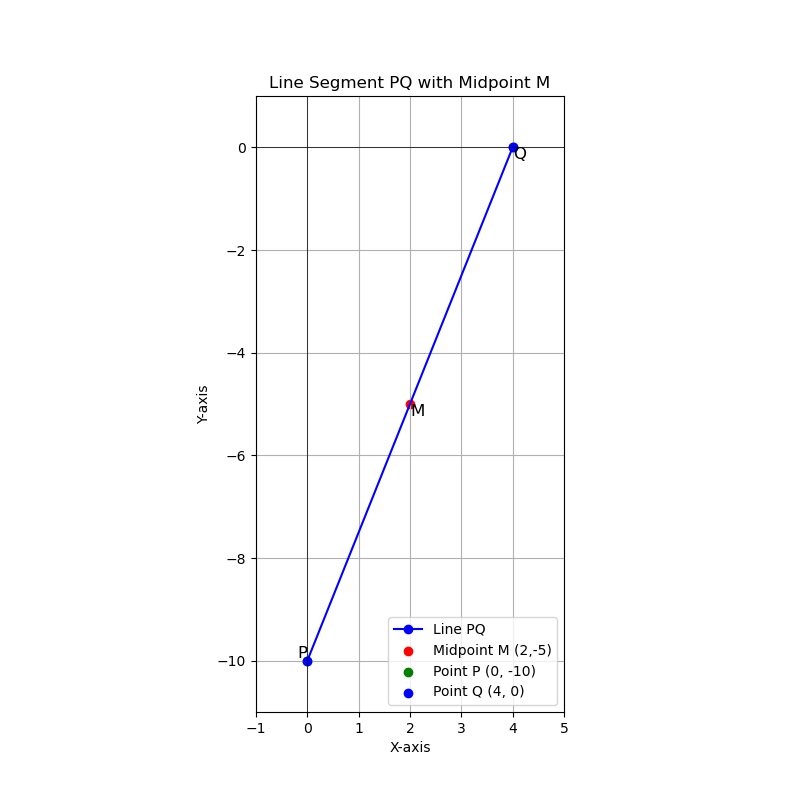
\includegraphics[width=0.7\textwidth]{Figure_1.png}
\caption{Plot showing points $ P $, $ Q $, and midpoint $ M $}
\label{fig:graph}
\end{figure}
\end{frame}

\begin{frame}[fragile]
\frametitle{C Code}
\begin{lstlisting}[language=C, basicstyle=\ttfamily\small, keywordstyle=\color{blue}]
#include <math.h>
#include <stdio.h>
#include <stdlib.h>
#include <string.h>
#include <unistd.h>
#include <sys/socket.h>
#include <netinet/in.h>

#include "libs/matfun.h"
#include "libs/geofun.h"
int main ()  {
    double **P,**Q,**M;
    P=createMat(2,1);
    Q=createMat(2,1);
    M=createMat(2,1);
    P[0][0]=0;        
    Q[1][0]=0;
    M[0][0]=2;
    M[1][0]=-5;

\end{lstlisting}
\end{frame}

\begin{frame}[fragile]

\begin{lstlisting}[language=C, basicstyle=\ttfamily\small, keywordstyle=\color{blue}]

    P[1][0]=2*(M[1][0]);
    Q[0][0]=2*(M[0][0]);

    FILE *file=fopen("output.dat","w");
    if (file == NULL)  {
        printf("Error opening file!\n");
        return 1;
    }

    fprintf(file,"P Q\n");
    fprintf(file,"%.2f %.2f\n",P[1][0],Q[0][0]);
    fclose(file);
    freeMat(P,2);
    freeMat(Q,2);
    freeMat(M,2);

    return 0;
}
\end{lstlisting}
\end{frame}

\begin{frame}[fragile]
\frametitle{python Code}
\begin{lstlisting}[language=python, basicstyle=\ttfamily\small, keywordstyle=\color{blue}]
#Code by GVV Sharma
#September 12, 2023
#Revised July 21, 2024
#released under GNU GPL
#Rank
import sys           #for path to external scripts
sys.path.insert
(0, '/home/teja-vardhan/Desktop/matgeo/codes/CoordGeo')        #path to my scripts
import numpy as np
import numpy.linalg as LA
import matplotlib.pyplot as plt
import matplotlib.image as mpimg

#local imports
from line.funcs import *
from triangle.funcs import *
from conics.funcs import circ_gen


\end{lstlisting}
\end{frame}

\begin{frame}[fragile]

\begin{lstlisting}[language=python, basicstyle=\ttfamily\small, keywordstyle=\color{blue}]

#if using termux
import subprocess
import shlex
#end if
data = np.genfromtxt
('output.dat', delimiter=' ', names=True)
x = data['P']
y = data['Q']

#Given points
P = np.array(([0,x])).reshape(-1,1)  
Q = np.array(([y,0])).reshape(-1,1)  
M = np.array(([2,-5])).reshape(-1,1) 
#Print rank 
print
(LA.matrix_rank(np.block([Q-P,M-P])))
#Generating all lines
x_PQ = line_gen(P,Q)
\end{lstlisting}
\end{frame}

\begin{frame}[fragile]

\begin{lstlisting}[language=python, basicstyle=\ttfamily\small, keywordstyle=\color{blue}]

#Plotting all lines
plt.plot(x_PQ[0,:],x_PQ[1,:],label='$PQ$')

#Labeling the coordinates
tri_coords = np.block([[P,Q,M]])
plt.scatter(tri_coords[0,:], tri_coords[1,:])
vert_labels = ['P','Q','M']
for i, txt in enumerate(vert_labels):
#plt.annotate(txt, # this is the text
plt.annotate
(f'{txt}\n({tri_coords[0,i]:.0f},
{tri_coords[1,i]:.0f})',
(tri_coords[0,i], tri_coords[1,i]),
            # this is the point to label
 textcoords="offset points",
            # how to position the text
xytext=(0,10),
            # distance from text to points (x,y)

\end{lstlisting}
\end{frame}

\begin{frame}[fragile]

\begin{lstlisting}[language=python, basicstyle=\ttfamily\small, keywordstyle=\color{blue}]
            
 ha='center') 
            # horizontal alignment can be left, right or center

# use set_position
ax = plt.gca()
ax.spines['top'].set_color('none')
ax.spines['left'].set_position('zero')
ax.spines['right'].set_color('none')
ax.spines['bottom'].set_position('zero')
#plt.xlabel('$x$')
#plt.ylabel('$y$')
plt.legend(loc='best')
plt.grid() # minor
plt.axis('equal')
plt.show()

\end{lstlisting}
\end{frame}

\end{document}


